\chapter{Research methodology}
\label{cha:methodology}

This chapter presents the research methodology on which the project will be based. In Section 3.1, the reference paper that the project initially seeks to reproduce will be discussed. In Section 3.2, the parallel hardware platforms that are available for experimentation will be described, along with the programming languages and models that they can support. In Section 3.3, the algorithm selected as a means of demonstrating parallelism on the target architectures will be described, with references to its origin and available implementations (both serial and parallel) from previous work. Section 3.6 discusses which of the programming models and languages reviewed in Chapter 2 are available for use in the hardware available for experimentation. In Section 3.5, the evaluation criteria for measuring the results obtained during the experiments performed as part of the project will be discussed.

\section{Approach to Portable Performance}

As mentioned during the introduction, performance portability will be attempted, based on the work done in~\cite{dolbeau2013one}. As mentioned in the previous chapter, the OpenCL framework offers suitable abstractions to create programs for a wide range of parallel architectures, but performance portability is not guaranteed.

The main experiment of the project will consist in understanding how the execution model configuration (NDRange, global and local work sizes, as described during Chapter 2) of a particular program may be tuned for different purposes, e.g. obtaining optimal performance for one particular architecture. This parameters may be configured globally in a program, so that all executed commands share the same configuration, or it may defined independently for each command to execute~\cite{khronos44opencl}.

Choosing a global work size is an easy task because, as explained in Chapter~\ref{cha:back}, it maps directly to the calculations that the algorithm must perform. The same situation happens with the NDRange details, because the number of dimensions that will be used is also problem-dependant, as different dimensions map better (or worse) to different kinds of problems.

The choice of a local work size has been identified as a more important factor for performance~\cite{Rosenberg2011}. In particular, it has been proposed that the local work size of a program can be tuned to get good performance from heterogeneous parallel architectures~\cite{dolbeau2013one}.

When left unspecified, OpenCL automatically selects a default local work size configuration that strives to~\cite{khronos44opencl}. This configuration is implementation-dependant and may only be known until runtime, either by using vendor tools like Intel's vTune~\cite{7_software.intel.com_2013}, or by using the \texttt{get\_local\_size} function defined by the OpenCL standard. It may not be the case that this default configuration is the optimal.

Manually choosing an adequate local work size is not a simple task, as there are many factors to consider. It is not always the case that choosing bigger or smaller local work sizes results in better performance, but because of the particularities of each OpenCL implementation and the technical specifications of each hardware device, there is not a defined methodology for finding an optimal size other than doing several experiments with different configurations~\cite{Rosenberg2011}~\cite{dolbeau2013one}.

Usually, this parameter is tuned for optimal performance on a particular model of parallel hardware. In this manner, specific versions of code are produced for every kind of architecture, and for particular models. Just as the CUDA model discussed in the previous chapter, which targets Nvidia GPUs only, performance portability is not guaranteed even when programming for the same type of architecture as the specifications of every new model may be very different.

By selecting an appropriate local work size, performance losses across all targets can be minimised and good parallel performance can still be obtained from different parallel architectures~\cite{dolbeau2013one}.

\section{Available hardware}

There are different architectures available on which to run experiments. While the following sections describe the details of these architectures, technical information has been summarised in Table~\ref{t:hwsum}. As mentioned during Chapter~\ref{cha:back}, it is important to cover modern and popular architectures. This project will perform experiments in CPU-based architectures (both multi-socket configurations and MIC devices), as well as GPU accelerators.

\begin{table}[!ht]
\begin{center}
\centerline{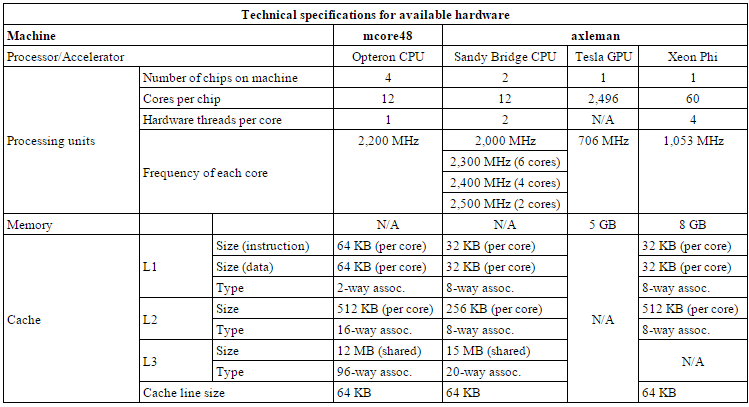
\includegraphics[width=\columnwidth]{img/hwsum}}
\caption[Summary of technical specifications of available hardware.]{Summary of technical specifications of available hardware, including main processors and accelerators. Configurations and frequencies of cores may be seen, along with details of the memory hierarchy of each chip.}
\label{t:hwsum}
\end{center}
\end{table}

%, 

\subsection{mcore48}

The mcore48 is a Dell machine composed of a four-chip board containing AMD Opteron 6174~\cite{amd} chips with 12 cores clocked at 2200 MHz. This CPU is based on the K10 microarchitecture. The L1 cache level has a Least Recently Used (LRU) replacement policy and a write-allocate policy, while both L2 and L3 cache levels have a pseudo LRU replacement policy. L3 cache level is shared, connected to all cores by a 3200 MHz HyperTransport bus.

The mcore48 has no addtional accelerators installed. The operating system running on the mcore48 is CentOS, version 6.5.

\subsection{axleman}

The axleman machine is more versatile than the mcore48. While in terms of CPUs it has a lower number of cores with lower frequencies and cache capacities, the CPUs in axleman have certain differences versus the CPUs on mcore48, as will be described in the following sections. It also comes equipped with two kinds of accelerators, making it a very important piece of hardware for the experiments that will be done during the project.

The operative system running on the axleman is CentOS, version 6.6.

\subsubsection{Sandy Bridge CPU}

Axleman is installed with two Intel Xeon E5-2620 x86-64 CPUs connected with Intel's QuickPath Interconnect (QPI) clocked at 3600 MHz, providing a point-to-point processor interconnect between these CPUs. This enables Non-Uniform Memory Access (NUMA). Programs may access data from both CPUs without any additional specifications and the programmer can think of the two processors as one big processor, even if memory accesses from one core to another have different access times (hence the NUMA classification).

The Xeon E5-2600 family of processors is based on the Sandy Bridge microarchitecture, released in 2011. It targets a 32 nanometer fabrication process. A single E5-2620 has six cores clocked at 2 GHz base frequency and at 2.5 GHz Turbo Boost frequency (depending on the number of cores working). It has support for HyperThreading (Intel's version of simultaneous multithreading), for a total of 12 hardware threads available~\cite{1_cpu-world.com_2015}. Cache sizes can be seen in Table~\ref{t:hwsum}.

This particular configuration of two CPUs installed on axleman will be referred to as the ``Sandy Bridge CPU" in the remainder of this document.

\subsubsection{Kepler GPU}

Axleman has additional accelerators installed. One of them is a Nvidia Tesla K20m GPU~\cite{6_gpuzoo.com_2015}, which has 2,496 cores and 5 GB of ram on-chip, organised in 20 blocks of 64M x 16 GDDR5~\cite{Nvidia2013}. The K20m is based on the Kepler GK110GL microarchitecture~\cite{Nvidia2012}. Details about the memory hierarchy can be seen in Table~\ref{t:hwsum}, though it works differently than that of CPU-based architectures. The Kepler GPU is connected to axleman with a PCIe x16 bus.

\subsubsection{Xeon Phi}

Axleman also has a MIC accelerator. The Xeon Phi model installed is the 5110P~\cite{3_cpu-world.com_2015}, with 60 cores, and uses a 22 nanometer fabrication process. Each core is a simple 64-bit Pentium processor, with an x86 ISA, clocked at 1,053 MHz. Each core also has a VPU capable of performing FMA operations with 512-bit SIMD vector registers. Because of 4-way multithreading, the Xeon Phi has a total of 240 hardware threads available. Cache and memory details may be consulted in Table~\ref{t:hwsum}, as defined in~\cite{5_intel_ark_productspecs_2015} and~\cite{4_software.intel.com_2012}.

The ``Xeon Phi", as the Xeon Phi model 5110P that is installed on axleman will be referred to from this point forward, is connected to axleman by PCIe x16.

\section{Algorithm selection: Shallow water simulation}

An algorithm will be used which is:
\begin{itemize}

\item Performance-relevant (a building block for other algorithms, universally used and actively surveyed in the literature).

\item Capable of demonstrating common bottlenecks in parallel computing.

\item Simple enough to provide reasonable modifications that increase its performance in heterogeneous architectures.

\item Interesting, such that optimisations may be useful for the continuous development of science.

\end{itemize}

Previous work in this domain has used a shallow water simulation as part of climate modelling. It presents opportunities for parallelism which have also been studied on the same (or very similar) hardware that was listed on this chapter, as seen in~\cite{pappas2012} and in~\cite{Cheng2014}.

\subsection{Complexity analysis}

The algorithm presents quadratic space and time complexities.

\begin{table}[!h]
\begin{center}
\centerline{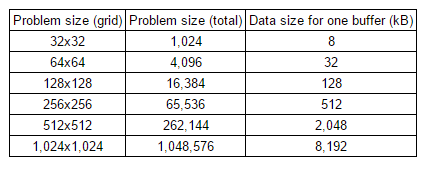
\includegraphics[width=3.5in]{img/problemsizescaling}}
\caption{Shallow water space complexity details.}
\label{t:space}
\end{center}
\end{table}


\begin{figure}[!h]
\begin{center}
\centerline{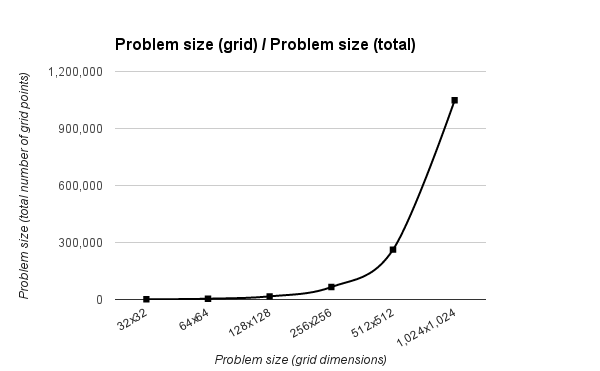
\includegraphics[width=5.5in]{img/problemsizeplot}}
\caption{Shallow water space complexity scalability plot.}
\label{f:spaceplot}
\end{center}
\end{figure}


\subsection{Code versions available from previous work}

The original serial Fortran version of the shallow water simulation used in this project was written by Paul N. Swarztrauber in 1984. The shallow water model is based on previous work from 1975~\cite{sadourny1975dynamics}. The performance of this version, as well as other parallel implementations, was thoroughly studied at the time of its creation~\cite{mcbryan1988new}. A port of this serial version to the C language was provided by Graham Riley (project supervisor) for this project.

There exist OpenMP and OpenCL versions created during the work done in~\cite{pappas2012}. The OpenCL version was specifically tuned for performance on an Nvidia Fermi GPU (a generation older than the currently installed Kepler GPU). As mentioned in Chapter~\ref{cha:back}, OpenCL does not aim for nor guarantee performance portability, so work may be needed to correctly exploit the performance achievable by the hardware currently available.

\section{Programming languages and available compilers}

The main platform in which to evaluate parallel performance will be OpenCL. As mentioned in~\cite{dolbeau2013one}, the OpenCL framework offers the unique opportunity to target different parallel architectures without changes to the code.

The code running on the host which will create the necessary contexts to run the kernels is written in C. The kernels, which are the pieces of code running on the device, are written in OpenCL's own C subset.

The available C/C++, Fortran, OpenCL and additional compilers and their versions for each piece of available hardware previously described can be seen in Table~\ref{t:compilers}. Axleman provides more varied compiler options relevant for the project, including OpenACC (though the current version only has support for Nvidia GPU accelerators, newer versions also support the Xeon Phi), while the Intel Fortran compiler in the mcore48 supports the newest version of OpenMP (which has accelerator support).

\begin{table}[!h]
\begin{center}
\centerline{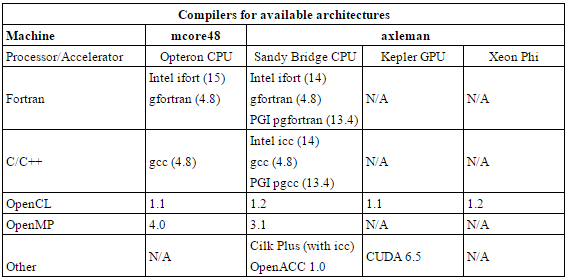
\includegraphics[width=\columnwidth]{img/compilers}}
\caption{Compilers for available architectures.}
\label{t:compilers}
\end{center}
\end{table}

\section{Evaluation}

Execution time ($T$) will be measured from parallel versions of the program running on the different architectures available. Performance will be measured as the inverse of time ($R = \frac{1}{T}$). Speedup will be calculated using Amdalh's Law~\cite{eager1989speedup} against a reference serial version (C, Fortran or OpenCL).

Execution time spent during memory allocations, either in the host or the device, or during memory transfers from the main memory to a device (and viceversa) will not be considered as the interest of the project lies in evaluating floating-point calculation performance. Memory allocations are traditionally complex~\cite{arpaci2012operating} and costly~\cite{detlefs1994memory} and hard to predict in terms of time of execution, mainly because of hardware and operating system performance techniques~\cite{herter2014timing}. Memory transfers, as explained during Chapter~\ref{cha:back}, are slow when considering that the accelerators on axleman are connected to a PCIe bus. Both factors provide additional overheads not directly related to the floating-point performance of the cores that will execute the program and perform the actual calculations.

The current version of the program will also make use of double-precision floating-point numbers. As evaluated in~\cite{pappas2012}, using single-precision variables provides better performance, at least on GPU devices. TODO less precise??? ASK GRAHAM!

Measuring performance using the specific roofline model~\cite{williams2009roofline} for each piece of parallel hardware available is to be considered for this project as well, provided enough time remains after experimentation. The roofline model is able to provide a visual representation of the achieved performance, while referencing directly vendor specifications and extensive benchmarking on a device, measuring performance in floating-point operations per second.

Various problem sizes for the shallow water simulation will be considered in order to better understand parallel hardware behaviour under different memory requirements. These problem size choices, which map directly to the global work size of an OpenCL program, might also affect the possible local work sizes available for experimentation for OpenCL versions of the program.

The OpenCL version will be tuned for specific architectures, varying the work-group dimensions as explained in this chapter. Another tuned version able to obtain reasonable speedup from heterogeneous architectures without changing the code will be sought. The initial search space of work-group dimensions configurations to experiment with is the same considered in~\cite{dolbeau2013one}, also listed in Table~\ref{t:wg}, but more fine-grained configurations may also be attempted.

\begin{table}[!h]
\begin{center}
\centerline{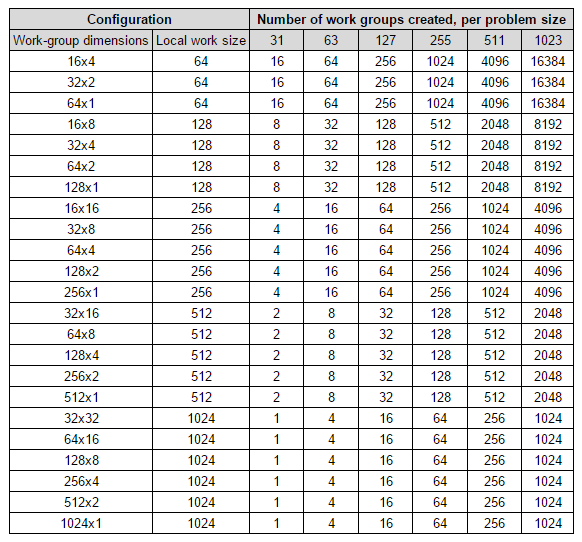
\includegraphics[width=5in]{img/wg}}
\caption{Work-group dimensions configurations for initial experimentation.}
\label{t:wg}
\end{center}
\end{table}

\begin{figure}[!h]
\begin{center}
\centerline{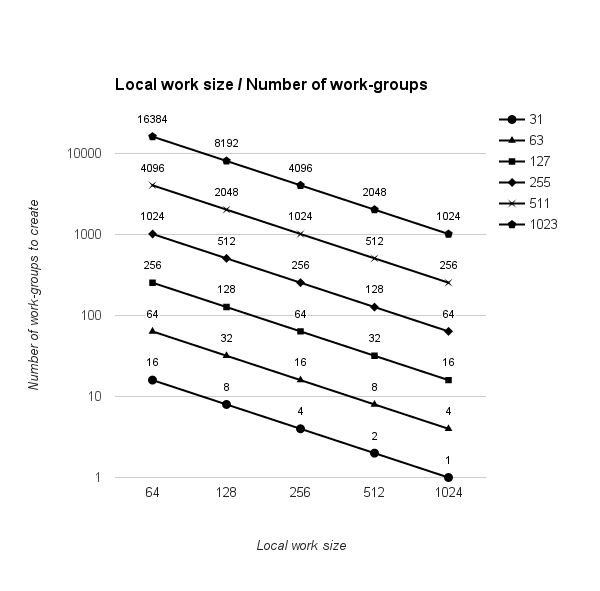
\includegraphics[width=5.2in]{img/wgplot}}
\caption{Work-group dimensions configurations for initial experimentation.}
\label{f:wgplot}
\end{center}
\end{figure}

The project will also seek to improve the performance of the current OpenCL version running on the Xeon Phi accelerator following the methodology of~\cite{7_software.intel.com_2014}, since the current version is not optimal~\cite{Cheng2014}~\cite{7_farber_2012}. For this, an attempt to understand the performance of this version in terms of its overheads will be made, though the inherent difficulty of tuning for performance is to be considered a priori~\cite{riley1997performance}.

% TODO The production of a new version in another programming language that can better exploit parallelism from this accelerator might also be considered.

Because of many different factors, execution time of repetitions of computational experiments tend to differ from one another, even under the same experimental conditions, sometimes significantly~\cite{nogueira2014experimental}. For this reason, the results obtained during the project will be evaluated to be statistically significant by measuring the square-mean error of 10 repetitions of executions under the same experimental conditions.

\section{Summary}

In this chapter, research and evaluation methodology for this project has been explained. The reference literature on which the project is based has been discussed in detail, with analysis in the context of the hardware available for experimentation and the programming models and languages which are supported by it. It is important to consider all previous work done in parallel implementations of shallow water simulations in order to advance research in performance portability, while maintaining a scientific approach to evaluate the results obtained.
